% !TeX program = pdflatex
\documentclass[10pt,aspectratio=169]{beamer}

% Metropolis theme
\usetheme[progressbar=frametitle,numbering=fraction]{metropolis}

\usepackage{amsmath,amssymb}
\usepackage{booktabs}
\usepackage{graphicx}
\usepackage{xcolor}
\usepackage{hyperref}

\usepackage{tikz}
\usepackage{etoolbox}
\usetikzlibrary{arrows.meta,positioning}
% --- put once in your preamble (optional, but nice) ---
\newcommand{\fin}[1]{\textcolor{blue}{\texttt{#1}}}
\newcommand{\eng}[1]{\textcolor{black}{\texttt{#1}}}
% ------------------------------------------------------------

% --- SQL highlighting ---
\newcommand{\sqlk}[1]{\textcolor{blue}{#1}}

\usepackage{listings}
\definecolor{dkgreen}{rgb}{0,0.6,0}
\definecolor{gray}{rgb}{0.5,0.5,0.5}
\definecolor{mauve}{rgb}{0.58,0,0.82}

\lstdefinestyle{sqlite}{
  language=SQL,
  morekeywords={
    TEXT,REAL,ROUND,CHAR,VARCHAR,INT,INTEGER,NUMERIC,DECIMAL,BOOLEAN,DATE,TIMESTAMP,
    PRAGMA,FOREIGN,PRIMARY,KEY,REFERENCES,DEFAULT,UNIQUE,CHECK,NOT,NULL,
    CREATE,ALTER,DROP,TABLE,VIEW,INDEX,
    GRANT,REVOKE,ROLE,WITH,OPTION,ALL,PRIVILEGES,CONNECT,EXECUTE,
    BEGIN,START,TRANSACTION,COMMIT,ROLLBACK,WORK,
    ISOLATION,LEVEL,SERIALIZABLE,REPEATABLE,READ,COMMITTED,UNCOMMITTED,
    CASCADE,RESTRICT,SET
  },
  basicstyle={\small\ttfamily},
  keywordstyle=\color{blue},
  commentstyle=\color{dkgreen},
  stringstyle=\color{mauve},
  numbers=none,
  showstringspaces=false,
  breaklines=true,
  breakatwhitespace=true,
  columns=flexible,
  tabsize=3,
  frame=single,
  rulecolor=\color{gray},
  xleftmargin=0.0em,
  framexleftmargin=0.0em,
  framexrightmargin=-1em,
  frameround=tttt,
}
\lstnewenvironment{codesql}{\lstset{style=sqlite}}{}

% Convenience
\newcommand{\partslide}[2]{%
  \begin{frame}[plain]
    \vfill
    {\Huge\textbf{#1}}\\[0.6em]
    {\Large #2}
    \vfill
  \end{frame}
}

\title{Database Programming in SQL -- Part II (continued)}
\subtitle{DDL, Access Control (DCL) \& Transactions (TxCL) \; (90 min)}
\author{Michael Emmerich}
\date{\today}

\begin{document}

\maketitle

% ------------------------------------------------------------
\begin{frame}{Roadmap (today)}
\begin{columns}[T,onlytextwidth]
\column{0.50\textwidth}
\textbf{1) DDL: schema \& integrity (30 min)}
\begin{itemize}
  \item Data types in practice
  \item Constraints: \sqlk{PRIMARY KEY}, \sqlk{FOREIGN KEY}, \sqlk{NOT NULL}, \sqlk{UNIQUE}, \sqlk{CHECK}, \sqlk{DEFAULT}
  \item \sqlk{ALTER TABLE} and schema evolution
  \item Views and indexes (what/why)
\end{itemize}

\column{0.50\textwidth}
\textbf{2) DCL \& TxCL (60 min)}
\begin{itemize}
  \item Access rights: roles, \sqlk{GRANT}, \sqlk{REVOKE}
  \item Transactions: \sqlk{BEGIN}/\sqlk{COMMIT}/\sqlk{ROLLBACK}
  \item ACID, isolation anomalies, isolation levels
  \item Locking, 2PL, deadlocks (conceptual)
\end{itemize}
\end{columns}
\end{frame}

% ------------------------------------------------------------
\begin{frame}{Connection to last lecture (2 min recap)}
\begin{itemize}
  \item Last time: querying data (\sqlk{SELECT}/\sqlk{WHERE}), joins, set operations, aggregation.
  \item Today: how we \emph{define} the structure, protect data, and keep it correct under concurrency.
\end{itemize}
\vspace{1mm}
\begin{block}{Mental model}
\medskip

\small
$\Rightarrow$\textbf{Schema (DDL)} says what data \emph{may exist}.\\ \quad\quad
$\Rightarrow$\textbf{Rights (DCL)} say who \emph{may do what}.\\ \quad\quad\quad
$\Rightarrow$\textbf{Transactions (TxCL)} say how concurrent changes stay \emph{correct}.
\end{block}
\end{frame}

% ======================= Part A: DDL =========================
\partslide{Part A}{Defining database structure (DDL) and Data Updates (DML)}

% ------------------------------------------------------------
\begin{frame}{SQL data types you will see often}
\small
SQL is strongly typed: each column has a declared type.
\vspace{1mm}
\begin{center}
\begin{tabular}{@{}lll@{}}
\toprule
\textbf{Type family} & \textbf{Examples} & \textbf{Typical use}\\
\midrule
Strings & \texttt{CHAR(n)}, \texttt{VARCHAR(n)}, \texttt{TEXT} & IDs, names, free text\\
Integers & \texttt{INT}, \texttt{INTEGER} & counts, years, quantities\\
Decimals & \texttt{NUMERIC(p,s)}, \texttt{DECIMAL(p,s)} & money, measurements\\
Booleans & \texttt{BOOLEAN} & flags, on/off states\\
Dates/times & \texttt{DATE}, \texttt{TIMESTAMP} & timestamps, events\\
\bottomrule
\end{tabular}
\end{center}
\vspace{1mm}
\footnotesize Practical note: exact type behavior depends on DBMS; always check your product's documentation.
\end{frame}

% ------------------------------------------------------------
\begin{frame}[fragile]{DDL recap: \sqlk{CREATE TABLE} (structure + rules)}
\small
\begin{itemize}
  \item Tables define columns, data types, and constraints.
  \item Constraints are the \textbf{first line of defense} for data quality.
\end{itemize}
\vspace{1mm}

\begin{lstlisting}[style=sqlite,basicstyle=\scriptsize\ttfamily]
CREATE TABLE CUSTOMER(
  customer_id   CHAR(4)      PRIMARY KEY,
  customer_name VARCHAR(15)  NOT NULL,
  city          VARCHAR(10),
  customer_type CHAR(1),
  district      CHAR(1)
);

CREATE TABLE INVOICE(
  invoice_id     CHAR(4)     PRIMARY KEY,
  year           INT,
  invoice_total  INT         CHECK (invoice_total >= 0),
  status         VARCHAR(2)  DEFAULT 'OK',
  customer_id    CHAR(4)     NOT NULL,
  FOREIGN KEY(customer_id) REFERENCES CUSTOMER(customer_id)
);
\end{lstlisting}
\end{frame}



% ------------------------------------------------------------
\begin{frame}[fragile]{Keys and referential integrity: \sqlk{PRIMARY KEY} + \sqlk{FOREIGN KEY}}
\small
\begin{columns}[T,onlytextwidth]
\column{0.52\textwidth}
\textbf{Composite primary key (relationship table)}
\begin{lstlisting}[style=sqlite,basicstyle=\scriptsize\ttfamily]
CREATE TABLE INVOICE_LINE(
  invoice_id   CHAR(4),
  product_id   CHAR(4),
  quantity     INT CHECK (quantity > 0),
  PRIMARY KEY (invoice_id, product_id),
  FOREIGN KEY (invoice_id) REFERENCES INVOICE(invoice_id) ON DELETE CASCADE,
  FOREIGN KEY (product_id) REFERENCES PRODUCT(product_id) ON DELETE SET NULL
);
\end{lstlisting}

\column{0.48\textwidth}
\textbf{Referential actions (idea)}
\begin{itemize}
  \item \sqlk{RESTRICT}: deny update/delete in parent
  \item \sqlk{ON DELETE SET NULL}: null Foreign Key in child
  \item \sqlk{ON DELETE CASCADE}: propagate change/delete to child
  \item \sqlk{ON DELETE SET DEFAULT}: assign default value
\end{itemize}
\vspace{1mm}
\footnotesize Exact availability and defaults depend on the DBMS.
\end{columns}
\end{frame}

% ------------------------------------------------------------
\begin{frame}[fragile]{Column constraints beyond keys}
\small
\begin{itemize}
  \item \sqlk{DEFAULT} sets a value if none is provided.
  \item \sqlk{NOT NULL} forbids missing values.
  \item \sqlk{UNIQUE} forbids duplicates.
  \item \sqlk{CHECK} enforces domain/business rules.
\end{itemize}

\vspace{1mm}
\begin{lstlisting}[style=sqlite,basicstyle=\scriptsize\ttfamily]
CREATE TABLE CUSTOMER(
  customer_id   CHAR(4)      PRIMARY KEY,
  customer_name VARCHAR(15)  NOT NULL,
  email         VARCHAR(50)  UNIQUE,
  customer_type CHAR(1)      DEFAULT 'A',
  district      CHAR(1)      CHECK (district IN ('I','L','1','2','3'))
);
\end{lstlisting}

\vspace{1mm}
\footnotesize Rule of thumb: encode the \emph{stable} rules in constraints; keep volatile rules in application logic.
\end{frame}

% ------------------------------------------------------------
\begin{frame}[fragile]{Schema evolution: \sqlk{ALTER TABLE}}
\small
\begin{itemize}
  \item Databases evolve: new requirements, new columns, stricter rules.
  \item \sqlk{ALTER TABLE} supports adding/dropping columns and constraints (syntax differs across DBMS).
\end{itemize}
\vspace{1mm}

\begin{lstlisting}[style=sqlite,basicstyle=\scriptsize\ttfamily]
-- Start minimal, then add constraints and columns
CREATE TABLE INVOICE_LINE(
  invoice_id CHAR(4),
  product_id CHAR(4)
);

ALTER TABLE INVOICE_LINE
  ADD COLUMN quantity INT;

-- In many DBMS (e.g., PostgreSQL) you can add constraints like this:
ALTER TABLE INVOICE_LINE
  ADD PRIMARY KEY (invoice_id, product_id);
\end{lstlisting}

\footnotesize Practical note: SQLite has limitations on ALTER TABLE compared to PostgreSQL/MySQL.
\end{frame}

% ------------------------------------------------------------
\begin{frame}[fragile]{Views and indexes: two important DB objects}
\begin{columns}[T,onlytextwidth]
\column{0.50\textwidth}
\textbf{View = stored query (no data stored)}
\begin{itemize}
  \item Simplifies common queries
  \item Helps define \textbf{fine-grained rights} (bridge to DCL)
\end{itemize}
\begin{lstlisting}[style=sqlite,basicstyle=\scriptsize\ttfamily]
CREATE VIEW v_east_customers AS
SELECT customer_name, city, customer_type
FROM CUSTOMER
WHERE district = 'I';

SELECT * FROM v_east_customers;
\end{lstlisting}

\column{0.48\textwidth}
\textbf{Index = faster search structure}
\begin{itemize}
  \item Speeds up \sqlk{WHERE}/\sqlk{JOIN}/\sqlk{ORDER BY} patterns
  \item Costs extra space and slows inserts/updates
\end{itemize}
\begin{lstlisting}[style=sqlite,basicstyle=\scriptsize\ttfamily]
CREATE INDEX customer_name_idx
ON CUSTOMER(customer_name);

DROP INDEX customer_name_idx;
\end{lstlisting}
\end{columns}
\end{frame}

% ------------------------------------------------------------
\begin{frame}[fragile]{Views: stored queries for reuse, rights, and derived data}
\small
\textbf{View = stored query (typically no data stored)}
\begin{itemize}
  \item Simplifies common queries and hides complexity
  \item Helps define \textbf{fine-grained access rights} (expose only selected columns/rows)
  \item Can provide \textbf{derived attributes} and \textbf{unit conversions}
\end{itemize}

\vspace{1mm}
\textbf{Example (SQLite): derived attributes + unit conversion}
\begin{lstlisting}[style=sqlite,basicstyle=\scriptsize\ttfamily]
-- Assume table CITIZEN(citizen_id, name, city, size_cm, birthdate)

CREATE VIEW v_citizen_profile AS
SELECT
  citizen_id,
  city,
  ROUND(size_cm / 30.48, 2) AS size_ft,  -- cm -> feet
  CAST((julianday('now') - julianday(birthdate)) / 365.25 AS INT) AS age_years
FROM CITIZEN;

SELECT * FROM v_citizen_profile;
\end{lstlisting}

\vspace{1mm}
\textbf{Privacy idea: aggregates make individual data disappear (public health style)}
\begin{lstlisting}[style=sqlite,basicstyle=\scriptsize\ttfamily]
CREATE VIEW v_city_health_stats AS
SELECT
  city,
  ROUND(AVG(size_cm), 1) AS avg_size_cm,
  ROUND(AVG(size_cm / 30.48), 2) AS avg_size_ft
FROM CITIZEN
GROUP BY city;
\end{lstlisting}
\end{frame}


% ------------------------------------------------------------
\begin{frame}[fragile]{Indexes: faster search structures (with trade-offs)}
\small
\textbf{Index = auxiliary structure to speed up lookups}
\begin{itemize}
  \item Speeds up \sqlk{WHERE} / \sqlk{JOIN} / \sqlk{ORDER BY}
  \item Costs extra space and can slow \sqlk{INSERT}/\sqlk{UPDATE}/\sqlk{DELETE}
\end{itemize}

\vspace{1mm}
\textbf{Common index types (concept)}
\begin{itemize}
  \item \textbf{Sorted list by attribute values}: fast search, but updates can be expensive
  \item \textbf{B+ tree}: keeps keys sorted, supports efficient updates, and supports \textbf{range queries}
  \item \textbf{Hash index}: use a hash function to map key $\rightarrow$ bucket/page; great for equality lookups,
        but not for ranges
\end{itemize}

\vspace{-2mm}
\textbf{Example: range query (benefits from B+ tree-like indexing)}
\begin{lstlisting}[style=sqlite,basicstyle=\scriptsize\ttfamily]
CREATE INDEX citizen_birthdate_idx
ON CITIZEN(birthdate);

-- Range query: citizens born between 1973 and 1993
SELECT citizen_id, birthdate
FROM CITIZEN
WHERE birthdate BETWEEN '1973-01-01' AND '1993-12-31';
\end{lstlisting}
\end{frame}


% ------------------------------------------------------------
\begin{frame}{From DDL to DML: changing the data}
\small
After \sqlk{CREATE TABLE}, we usually start manipulating rows using \textbf{DML}:
\vspace{1mm}
\begin{itemize}
  \item \sqlk{INSERT} = add new rows
  \item \sqlk{UPDATE} = modify existing rows
  \item \sqlk{DELETE} = remove rows
\end{itemize}
\vspace{1mm}
\begin{block}{CRUD mapping (common in apps)}
\medskip

\footnotesize
Create (rows) $\rightarrow$ \sqlk{INSERT}\quad
Read $\rightarrow$ \sqlk{SELECT}\quad
Update $\rightarrow$ \sqlk{UPDATE}\quad
Delete $\rightarrow$ \sqlk{DELETE}
\end{block}
\end{frame}

% ------------------------------------------------------------
\begin{frame}[fragile]{\sqlk{INSERT}: adding rows}
\small
\begin{itemize}
  \item Always prefer the \textbf{explicit column list} (robust to schema changes).
  \item Columns not mentioned become \texttt{NULL} or their \sqlk{DEFAULT}, if defined.
\end{itemize}
\vspace{1mm}

\begin{lstlisting}[style=sqlite,basicstyle=\scriptsize\ttfamily]
-- Insert one customer
INSERT INTO CUSTOMER (customer_id, customer_name, city, customer_type, district)
VALUES ('C001', 'Anna', 'Jyvaskyla', 'A', 'I');

-- Insert an invoice (status uses DEFAULT 'OK')
INSERT INTO INVOICE (invoice_id, year, invoice_total, customer_id)
VALUES ('I001', 2025, 120, 'C001');

-- Insert multiple rows (supported in most DBMS incl. PostgreSQL, MySQL, SQLite)
INSERT INTO CUSTOMER (customer_id, customer_name, city, customer_type, district)
VALUES
  ('C002', 'Ben',  'Turku',     'A', 'L'),
  ('C003', 'Cleo', 'Helsinki',  'B', '2');
\end{lstlisting}

\vspace{0.5em}
\footnotesize
Typical failure modes: duplicate \sqlk{PRIMARY KEY}, \sqlk{FOREIGN KEY} missing parent, \sqlk{CHECK} violated.
\end{frame}

% ------------------------------------------------------------
\begin{frame}[fragile]{\sqlk{UPDATE}: changing existing rows}
\small
\begin{itemize}
  \item \sqlk{UPDATE} changes \textbf{all rows that match} the \sqlk{WHERE} condition.
  \item \textbf{Without \sqlk{WHERE}}: you update \emph{every row} (common accident).
\end{itemize}
\vspace{1mm}

\begin{lstlisting}[style=sqlite,basicstyle=\scriptsize\ttfamily]
-- Mark an invoice as paid
UPDATE INVOICE
SET status = 'PA'
WHERE invoice_id = 'I001';

-- Correct a total (also demonstrates an expression)
UPDATE INVOICE
SET invoice_total = invoice_total + 10
WHERE year = 2025
  AND status = 'OK';

-- Update multiple columns at once
UPDATE CUSTOMER
SET city = 'Tampere',
    district = '1'
WHERE customer_id = 'C002';
\end{lstlisting}

\vspace{0.5em}
\footnotesize Tip: do a \sqlk{SELECT ... WHERE ...} first to verify which rows will be affected.
\end{frame}

% ------------------------------------------------------------
\begin{frame}[fragile]{\sqlk{DELETE}: removing rows}
\small
\begin{itemize}
  \item \sqlk{DELETE} removes \textbf{rows}, not table structure (that would be \sqlk{DROP TABLE}).
  \item \textbf{Without \sqlk{WHERE}}: you delete \emph{every row}.
  \item Foreign keys may block deletion (e.g., \sqlk{RESTRICT}) or propagate it (\sqlk{CASCADE}).
\end{itemize}
\vspace{1mm}

\begin{lstlisting}[style=sqlite,basicstyle=\scriptsize\ttfamily]
-- Delete one invoice (only works if no referencing rows, or CASCADE is set)
DELETE FROM INVOICE
WHERE invoice_id = 'I001';

-- Delete all "test" customers (example condition)
DELETE FROM CUSTOMER
WHERE customer_name LIKE 'Test%';

-- Delete ALL rows (table remains!)
DELETE FROM INVOICE;
\end{lstlisting}

\vspace{0.5em}
\footnotesize In practice: deletions are often done inside transactions, and sometimes replaced by “soft delete”
(e.g., a column \texttt{is\_active}).
\end{frame}


% ======================= Part B: DCL =========================
\partslide{Part B}{Defining access rights (DCL)}

% ------------------------------------------------------------
\begin{frame}{Roles, users, and privileges (concept)}
\small
\begin{itemize}
  \item SQL standard abstracts users/groups as \textbf{roles}.
  \item Every DB object has an \textbf{owner} (typically the creator).
  \item Owners can grant/revoke privileges to other roles.
\end{itemize}
\vspace{1mm}

\begin{block}{Typical privileges}
\footnotesize
\begin{tabular}{@{}ll@{}}
\toprule
\textbf{Privilege} & \textbf{Allows}\\
\midrule
\texttt{CONNECT} & connect to database\\
\texttt{SELECT} & read data\\
\texttt{INSERT} & insert rows\\
\texttt{UPDATE} & modify rows/columns\\
\texttt{DELETE} & delete rows\\
\texttt{EXECUTE} & execute routines\\
\texttt{ALL PRIVILEGES} & all above except \texttt{CONNECT}\\
\bottomrule
\end{tabular}
\end{block}
\end{frame}

% ------------------------------------------------------------
\begin{frame}[fragile]{\sqlk{GRANT}: giving rights (with delegation option)}
\small
\begin{columns}[T,onlytextwidth]
\column{0.55\textwidth}
\textbf{General form}
\begin{codesql}
GRANT privilege[, privilege]*
ON object
TO role[, role]*
[WITH GRANT OPTION];
\end{codesql}

\textbf{Example: allow reading and updating, and allow re-granting}
\begin{codesql}
GRANT SELECT, UPDATE
ON INVOICE
TO analyst_role
WITH GRANT OPTION;
\end{codesql}

\column{0.45\textwidth}
\textbf{Column-level grants (fine-grained)}
\begin{codesql}
GRANT UPDATE (invoice_total, status)
ON INVOICE
TO billing_clerk;
\end{codesql}

\vspace{1mm}
\footnotesize Tip: combine with \textbf{views} to expose only selected columns/rows.
\end{columns}
\end{frame}

% ------------------------------------------------------------
\begin{frame}[fragile]{Roles can be granted to roles (hierarchies)}
\small
\begin{itemize}
  \item Role hierarchies help manage many users: one grant updates many accounts.
  \item Creating users/roles is DBMS-specific (example shown in PostgreSQL style).
\end{itemize}

\vspace{1mm}
\begin{lstlisting}[style=sqlite,basicstyle=\scriptsize\ttfamily]
-- PostgreSQL-like example:
CREATE ROLE masa
  WITH PASSWORD 'jkl0088'
  IN ROLE varastotyontekijat
  LOGIN
  VALID UNTIL 'May 8 11:30:00 2016';

-- Grant role to role (inherit privileges)
GRANT analyst_role TO intern_role;
\end{lstlisting}

\vspace{0.3em}
\footnotesize
\fin{varastotyontekijat}\footnote{Finnish (standard spelling): \emph{varastoty\"ontekij\"at} = “warehouse workers”.
Parts: \emph{varasto} = warehouse; \emph{ty\"ontekij\"a} = worker; \emph{-t} = plural.}
= \eng{warehouse\_workers}.

\end{frame}

% ------------------------------------------------------------
\begin{frame}[fragile]{\sqlk{REVOKE}: removing rights (and what happens downstream)}
\small
\begin{columns}[T,onlytextwidth]
\column{0.56\textwidth}
\textbf{General form}
\begin{codesql}
REVOKE [GRANT OPTION FOR] privilege[, privilege]*
ON object
FROM role[, role]*;
\end{codesql}

\textbf{Remove only delegation right}
\begin{codesql}
REVOKE GRANT OPTION FOR SELECT
ON INVOICE
FROM analyst_role;
\end{codesql}

\column{0.44\textwidth}
\textbf{Cascading effect (idea)}
\begin{itemize}
  \item If A granted to B \emph{with grant option}
  \item and B granted further to C,
  \item then revoking from B typically also removes the derived right from C.
\end{itemize}

\vspace{1mm}
\textbf{Best practice}
\begin{itemize}
  \item least privilege
  \item prefer views for fine-grained exposure
\end{itemize}
\end{columns}
\end{frame}

% ======================= Part C: TxCL =========================
\partslide{Part C}{Transaction control (TxCL)}

% ------------------------------------------------------------
\begin{frame}[fragile]{Transactions in SQL: the 3 core commands}
\small
\begin{itemize}
  \item A transaction groups 1..n operations into one logical unit of work.
  \item SQL transaction control uses:
\end{itemize}
\vspace{1mm}
\begin{codesql}
BEGIN [TRANSACTION];
-- ... your SELECT/INSERT/UPDATE/DELETE ...
COMMIT;   -- make changes permanent and visible
-- or
ROLLBACK; -- cancel changes of this transaction
\end{codesql}

\vspace{1mm}
\footnotesize Many systems also have \emph{autocommit} mode: each statement becomes its own transaction unless you BEGIN explicitly.
\end{frame}

% ------------------------------------------------------------
\begin{frame}{ACID: what DBMSs try to guarantee}
\small
\begin{block}{A -- Atomicity}
Either all operations succeed or none (failure triggers rollback).
\end{block}
\begin{block}{C -- Consistency}
Database moves from one consistent state to another (constraints + rules hold).
\end{block}
\begin{block}{I -- Isolation}
Concurrent transactions behave as if executed in some serial order.
\end{block}
\begin{block}{D -- Durability}
After commit, results persist even after crashes (within practical limits).
\end{block}
\end{frame}

% ------------------------------------------------------------
\begin{frame}[fragile]{Example (concept): guard a business rule with rollback}
\small
Business rule: bank account balance must not go below 0.
\vspace{1mm}

\begin{lstlisting}[style=sqlite,basicstyle=\scriptsize\ttfamily]
BEGIN TRANSACTION;
SELECT saldo
FROM tili
WHERE tilinro = :account_no;

-- if account not found: ROLLBACK;

UPDATE tili
SET saldo = saldo - :amount
WHERE tilinro = :account_no;

SELECT saldo
FROM tili
WHERE tilinro = :account_no;

-- if saldo < 0: ROLLBACK;

COMMIT;
\end{lstlisting}

\vspace{0.3em}
\footnotesize
\fin{tili}\footnote{Finnish: \emph{tili} = account (e.g., bank account, user account).}
= \eng{account},\;
\fin{tilinro}\footnote{Common abbreviation: \emph{tilinro} < \emph{tilinumero} = account number.
(\emph{numero} = number; \emph{nro} is a widely used Finnish abbreviation for “number”.)}
= \eng{account\_no},\;
\fin{saldo}\footnote{Finnish: \emph{saldo} = balance (current amount in an account).}
= \eng{balance}.

\footnotesize (Pseudo-code style: checks are done in the host program or via triggers.)
\end{frame}

% ------------------------------------------------------------
\begin{frame}{Isolation: what can go wrong with concurrency?}
\small
If transactions run in parallel, anomalies may violate the “as-if-serial” idea.

\vspace{1mm}
\begin{block}{Classic anomalies}
\begin{itemize}
  \item \textbf{Lost update}: two writers overwrite each other (final state misses one update).
  \item \textbf{Dirty read}: a transaction reads uncommitted changes from another transaction.
  \item \textbf{Non-repeatable read}: re-reading a row yields a different value (someone committed an update).
  \item \textbf{Phantom read}: re-running a range query yields different \emph{set of rows} (someone inserted/deleted in the range).
\end{itemize}
\end{block}
\end{frame}

% ------------------------------------------------------------
\begin{frame}[fragile]{Lost update (simple example)}
\small
Two transactions both add 20 to the same balance, but one update is lost.
\vspace{1mm}

\begin{center}
\begin{tabular}{@{}p{0.10\textwidth}p{0.43\textwidth}p{0.43\textwidth}@{}}
\toprule
\textbf{Time} & \textbf{T1} & \textbf{T2}\\
\midrule
$t_1$ & Read balance = 100  & --- \\
$t_2$ & ---                & Read balance = 100 \\
$t_3$ & Write balance = 120 & --- \\
$t_4$ & ---                & Write balance = 120 \\
\bottomrule
\end{tabular}
\end{center}

\vspace{1mm}
\begin{block}{Observation}
\small
Parallel result: 120.\quad Serial result First T1 then T2: 140.\quad
Isolation aims to prevent this mismatch.
\end{block}
\end{frame}

% ------------------------------------------------------------
\begin{frame}{Isolation levels (SQL standard idea)}
\small
Looser isolation can be faster but allows more anomalies.

\vspace{1mm}
\begin{center}
\begin{tabular}{@{}lccc@{}}
\toprule
\textbf{Isolation level} & \textbf{Dirty reads} & \textbf{Non-repeatable} & \textbf{Phantoms}\\
\midrule
\texttt{SERIALIZABLE} & no & no & no\\
\texttt{REPEATABLE READ} & no & no & yes\\
\texttt{READ COMMITTED} & no & yes & yes\\
\texttt{READ UNCOMMITTED} & yes & yes & yes\\
\bottomrule
\end{tabular}
\end{center}

\vspace{1mm}
\footnotesize Exact behavior can differ by DBMS; the table captures the \emph{standard} intent.
\end{frame}

% ------------------------------------------------------------
\begin{frame}{Concurrency control: how isolation is implemented (concept)}
\small
\begin{itemize}
  \item A \textbf{schedule} is the interleaving of operations of concurrent transactions.
  \item A schedule is \textbf{serializable} if it is equivalent to some serial order.
  \item DBMSs use techniques such as:
  \begin{itemize}
    \item \textbf{Locking} (common in classic RDBMS)
    \item \textbf{Timestamp ordering} (also common in some settings)
    \item \textbf{Optimistic vs pessimistic} strategies (high-level view)
  \end{itemize}
\end{itemize}
\end{frame}



% ------------------------------------------------------------
\begin{frame}{Two-phase locking (2PL): the key protocol}
\small
2PL structures each transaction into two phases:
\vspace{1mm}
\begin{block}{Expanding phase}
Acquire all needed locks (and promotions). Do \emph{not} release locks yet.
\end{block}
\begin{block}{Shrinking phase}
Release locks when they are no longer needed. Do \emph{not} acquire new locks.
\end{block}

\vspace{1mm}
\begin{itemize}
  \item 2PL + proper lock types aims for serializability.
  \item Stronger variants:
  \begin{itemize}
    \item \textbf{Conservative 2PL}: acquire all locks before doing anything. $\Rightarrow$ Avoids deadlocks
    \item \textbf{\underline{Strict 2PL}}: keep all write locks until commit/rollback.
    $\Rightarrow$ Avoids cascading rollback.
    \item \textbf{Strong strict 2PL}: keep all locks until commit/rollback.
  \end{itemize}
\end{itemize}



Papadimitriou, C. H. (1979). The serializability of concurrent database updates. Journal of the ACM (JACM), 26(4), 631-653.

\end{frame}

% ------------------------------------------------------------
\begin{frame}{Strict 2PL example: lock upgrade causes waiting}
\small
\textbf{Notation:} \texttt{S(X)} = shared (read) lock on item X,\;
\texttt{X(X)} = exclusive (write) lock,\;
\texttt{R(X), W(X)} = read/write.\;
\textbf{Strict 2PL:} locks are released only at \sqlk{COMMIT}/\sqlk{ROLLBACK}.

\vspace{1mm}
\begin{center}
\scriptsize
\begin{tabular}{@{}r l l p{0.36\textwidth}@{}}
\toprule
\textbf{Step} & \textbf{T1} & \textbf{T2} & \textbf{Lock state / comment}\\
\midrule
1  & \texttt{S(A)} &  & \texttt{S(A)} held by T1\\
2  & \texttt{R(A)} &  & read ok\\
3  & \texttt{X(A)} &  & upgrade ok (no other holders)\\
4  & \texttt{W(A)} &  & \texttt{X(A)} held by T1\\
5  &  & \texttt{S(B)} & \texttt{S(B)} held by T2\\
6  &  & \texttt{R(B)} & read ok\\
7  & \texttt{S(B)} &  & compatible: T1 also gets \texttt{S(B)}\\
8  & \texttt{R(B)} &  & read ok\\
9  & \texttt{X(B)} &  & \textbf{WAIT}: cannot upgrade while T2 holds \texttt{S(B)}\\
10 &  & \sqlk{COMMIT} & strict 2PL: T2 releases \texttt{S(B)} only now\\
11 & \texttt{X(B)} &  & upgrade granted\\
12 & \texttt{W(B)} &  & write ok\\
13 & \sqlk{COMMIT} &  & strict 2PL: T1 releases \texttt{X(A)}, \texttt{X(B)}\\
\bottomrule
\end{tabular}
\end{center}

\footnotesize
Takeaway: even a \emph{reader} (T2) can block a \emph{writer} (T1) under strict 2PL when the writer needs an \texttt{S$\rightarrow$X} upgrade.
\end{frame}




% ------------------------------------------------------------
\begin{frame}{Deadlocks: circular waiting for locks}
\small
\begin{itemize}
  \item Two-phase locking (2PL) helps isolation/serializability, but it can create \textbf{deadlocks}.
  \item A \textbf{deadlock} is a \textbf{cycle of waiting}: each transaction waits for a lock held by another.
  \item The situation does \emph{not} resolve by itself: the DBMS must abort (rollback) one transaction.
\end{itemize}

\vspace{1mm}
\begin{center}
\begin{tabular}{@{}l p{0.40\textwidth} p{0.40\textwidth}@{}}
\toprule
\textbf{Step} & \textbf{T1} & \textbf{T2}\\
\midrule
1 & X-lock(A) granted & \\
2 &  & X-lock(B) granted\\
3 & request X-lock(B) \emph{(blocked)} & \\
4 &  & request X-lock(A) \emph{(blocked)}\\
\midrule
 & \multicolumn{2}{l}{Now: T1 waits for B (held by T2) and T2 waits for A (held by T1) $\Rightarrow$ deadlock.}\\
\bottomrule
\end{tabular}
\end{center}

\footnotesize
Key idea: the \emph{wait-for} relation forms a cycle (T1 waits for T2, and T2 waits for T1).
\end{frame}


% In preamble:
% \usepackage{tikz}
% \usetikzlibrary{arrows.meta,positioning}

% ------------------------------------------------------------

\newcommand{\stickman}[2]{%
  % #1 x, #2 y
  \draw[line width=0.9pt] (#1,#2) circle (0.25);            % head
  \draw[line width=0.9pt] (#1,#2-0.25) -- (#1,#2-1.0);      % body
  \draw[line width=0.9pt] (#1,#2-0.45) -- (#1-0.45,#2-0.75);% left arm
  \draw[line width=0.9pt] (#1,#2-0.45) -- (#1+0.45,#2-0.75);% right arm
  \draw[line width=0.9pt] (#1,#2-1.0) -- (#1-0.4,#2-1.45);  % left leg
  \draw[line width=0.9pt] (#1,#2-1.0) -- (#1+0.4,#2-1.45);  % right leg
}
\begin{frame}{Deadlock (human edition)}
\centering
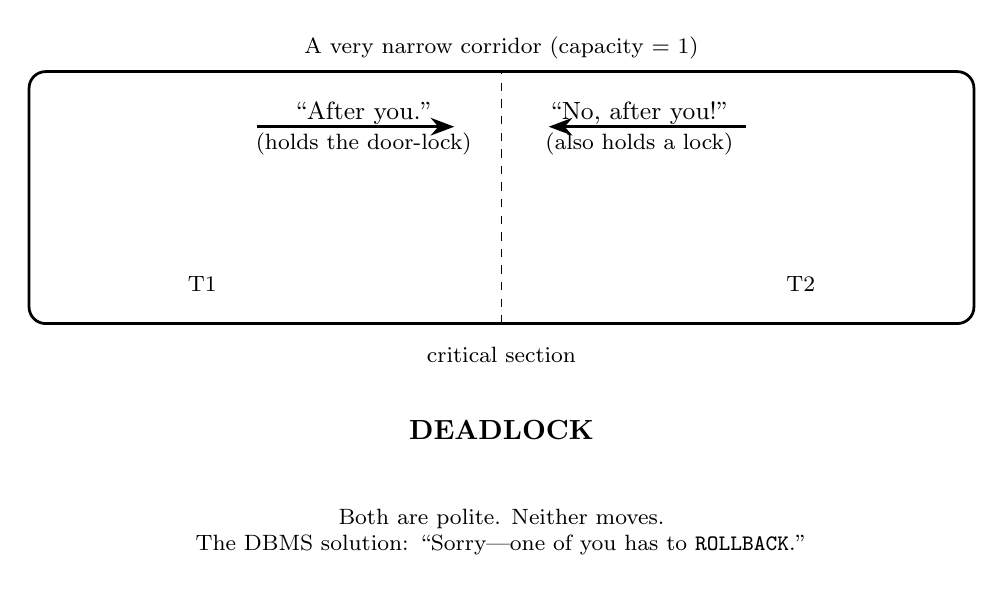
\begin{tikzpicture}[scale=1, every node/.style={font=\small}]
  % Corridor
  \draw[rounded corners=6pt, line width=1pt] (-6,-1.6) rectangle (6,1.6);
  \node[font=\footnotesize] at (0,1.9) {A very narrow corridor (capacity = 1)};

  % Center "blocked" zone
  \draw[dashed] (0,-1.6) -- (0,1.6);
  \node[font=\footnotesize] at (0,-2.0) {critical section};

  % Two simple men
  \stickman{-0.8}{0}
  \stickman{ 0.8}{0}
  \node at (-3.8,-1.1) {\footnotesize T1};
  \node at ( 3.8,-1.1) {\footnotesize T2};

  % Intent arrows
  \draw[-{Stealth[length=3mm]}, line width=1pt] (-3.1,0.9) -- (-0.6,0.9);
  \draw[-{Stealth[length=3mm]}, line width=1pt] ( 3.1,0.9) -- ( 0.6,0.9);

  % Speech bubbles (simple)
  \node[align=center] at (-1.75,0.875) {“After you.”\\ \footnotesize (holds the door-lock)};
  \node[align=center] at (1.75,0.875) {“No, after you!”\\ \footnotesize (also holds a lock)};

  % Deadlock label
  \node[font=\bfseries] at (0,-2.95) {DEADLOCK};
  \node[font=\footnotesize, align=center] at (0,-4.25)
    {Both are polite. Neither moves.\\
     The DBMS solution: “Sorry—one of you has to \texttt{ROLLBACK}.”};
\end{tikzpicture}
\end{frame}



% ------------------------------------------------------------
\begin{frame}{Deadlocks: typical handling strategies}
\small
\begin{columns}[T,onlytextwidth]
\column{0.5\textwidth}
\textbf{1) Prevention (avoid cycles)}
\begin{itemize}
  \item \textbf{Lock ordering}: always request locks in a fixed global order\\
        (e.g., by primary key, table order, or object id).
  \item \textbf{Timestamp priority protocols}:
  \begin{itemize}
    \item \textbf{wait-die}: \emph{older may wait}; \emph{younger aborts} if it would wait for older.
    \item \textbf{wound-wait}: \emph{older aborts (wounds) younger}; \emph{younger may wait} for older.
  \end{itemize}
\end{itemize}

\column{0.48\textwidth}
\textbf{2) Detection (allow, then resolve)}
\begin{itemize}
  \item DBMS maintains a \textbf{wait-for graph}.
  \item If there is a \textbf{cycle}, a deadlock is detected.
  \item DBMS chooses a \textbf{victim}, does \sqlk{ROLLBACK}, releases locks.
\end{itemize}

\vspace{1mm}
\textbf{3) Timeout (simple fallback)}
\begin{itemize}
  \item If a lock wait exceeds a threshold: abort + retry.
\end{itemize}
\end{columns}

\vspace{1mm}
\footnotesize
Practical takeaway: deadlocks are normal in concurrent systems; robust applications handle “transaction aborted” by retrying.
\end{frame}



% ------------------------------------------------------------
\begin{frame}[fragile]{In SQL: setting isolation level (typical pattern)}
\small
Syntax varies by DBMS, but the idea is:

\vspace{1mm}
\begin{codesql}
BEGIN;
-- (DBMS-specific) set isolation for this transaction:
SET TRANSACTION ISOLATION LEVEL SERIALIZABLE;

-- do work safely
SELECT ...;
UPDATE ...;

COMMIT;
\end{codesql}

\vspace{1mm}
\footnotesize Takeaway: you choose an isolation level to trade off speed vs anomalies.
\end{frame}

% ------------------------------------------------------------
% \begin{frame}{Mini-exercises for class (10 min)}
% \small
% \begin{enumerate}
%   \item Add a constraint: In \texttt{INVOICE}, enforce \texttt{invoice\_total >= 0} and status in \{\texttt{'OK'},\texttt{'PA'}\}.
%   \item Create a view \texttt{v\_customer\_public(customer\_id, city)} and explain why it is useful for access rights.
%   \item Explain which isolation level you would pick for:
%     \begin{itemize}
%       \item (a) a live dashboard that may tolerate slightly stale reads
%       \item (b) transferring money between accounts
%     \end{itemize}
% \end{enumerate}
% \end{frame}

% ------------------------------------------------------------
\begin{frame}{Summary}
\small
\begin{itemize}
  \item \textbf{DDL}: define structure + constraints; evolve schema via \sqlk{ALTER}; use \textbf{views} and \textbf{indexes}.
  \item \textbf{DCL}: manage access via roles and \sqlk{GRANT}/\sqlk{REVOKE}; prefer least privilege and views for fine-grained rights.
  \item \textbf{TxCL}: group operations into transactions; ACID; isolation levels; locking/2PL; deadlocks exist and are handled by the DBMS.
\end{itemize}
\end{frame}



\begin{frame}[fragile]{A friendly SQL bar joke summarizing the lecture}
\small

\begin{itemize}
  \item \textbf{DDL} walks into a bar and says: ``I would like to \texttt{CREATE TABLE}.''
  \item \textbf{DCL} replies (smiling): ``Only if I \texttt{GRANT} you permission.''
  \item \textbf{DML} jumps in: ``Great, I will \texttt{INSERT} some customers, \texttt{UPDATE} the bill, and \texttt{DELETE} the evidence.''
\end{itemize}

\vspace{2mm}
\textbf{A QUERY} squints at the menu and says:
\begin{lstlisting}[style=sqlite,basicstyle=\scriptsize\ttfamily]
SELECT beer
FROM fridge
WHERE cold = TRUE
ORDER BY foam DESC
LIMIT 1;
\end{lstlisting}

\vspace{1mm}
\textbf{TxCL} sighs (kindly): ``BEGIN... and if this gets messy, we ROLLBACK.''

\vspace{1mm}
\footnotesize
Kind reminder: be nice to your future self -- use transactions, and always leave the database consistent.

\end{frame}


\begin{frame}[plain]
\vfill
\centering
{\Large \textbf{Next up in the course}}\\[0.8em]
\begin{itemize}
  \item More query and data definition patterns and performance intuitions
  \item Interfacing a SQL database management system with a host programming language
  \item Practical exercises on your DBMS
\end{itemize}
\vfill
\end{frame}
\end{document}
